\chap{The runtime}{runtime}
\section{Notes}

There are multiple, possibly orthogonal issues.  Limit checks and garbage
collections are a little overloaded in their roles, because they also
support preemptive thread switching and interrupt handling.  Forcing
frontier to be 0 and hitting a limit check (even a zero byte limit check)
will invoke the GC, which will switch to the pending thread.

Recall that a limit check with bytes = 0 really means a check for LIMIT\_SLOP
bytes (currently LIMIT\_SLOP = 512).

\section{Bootstrap}

\figBegin
\centerline{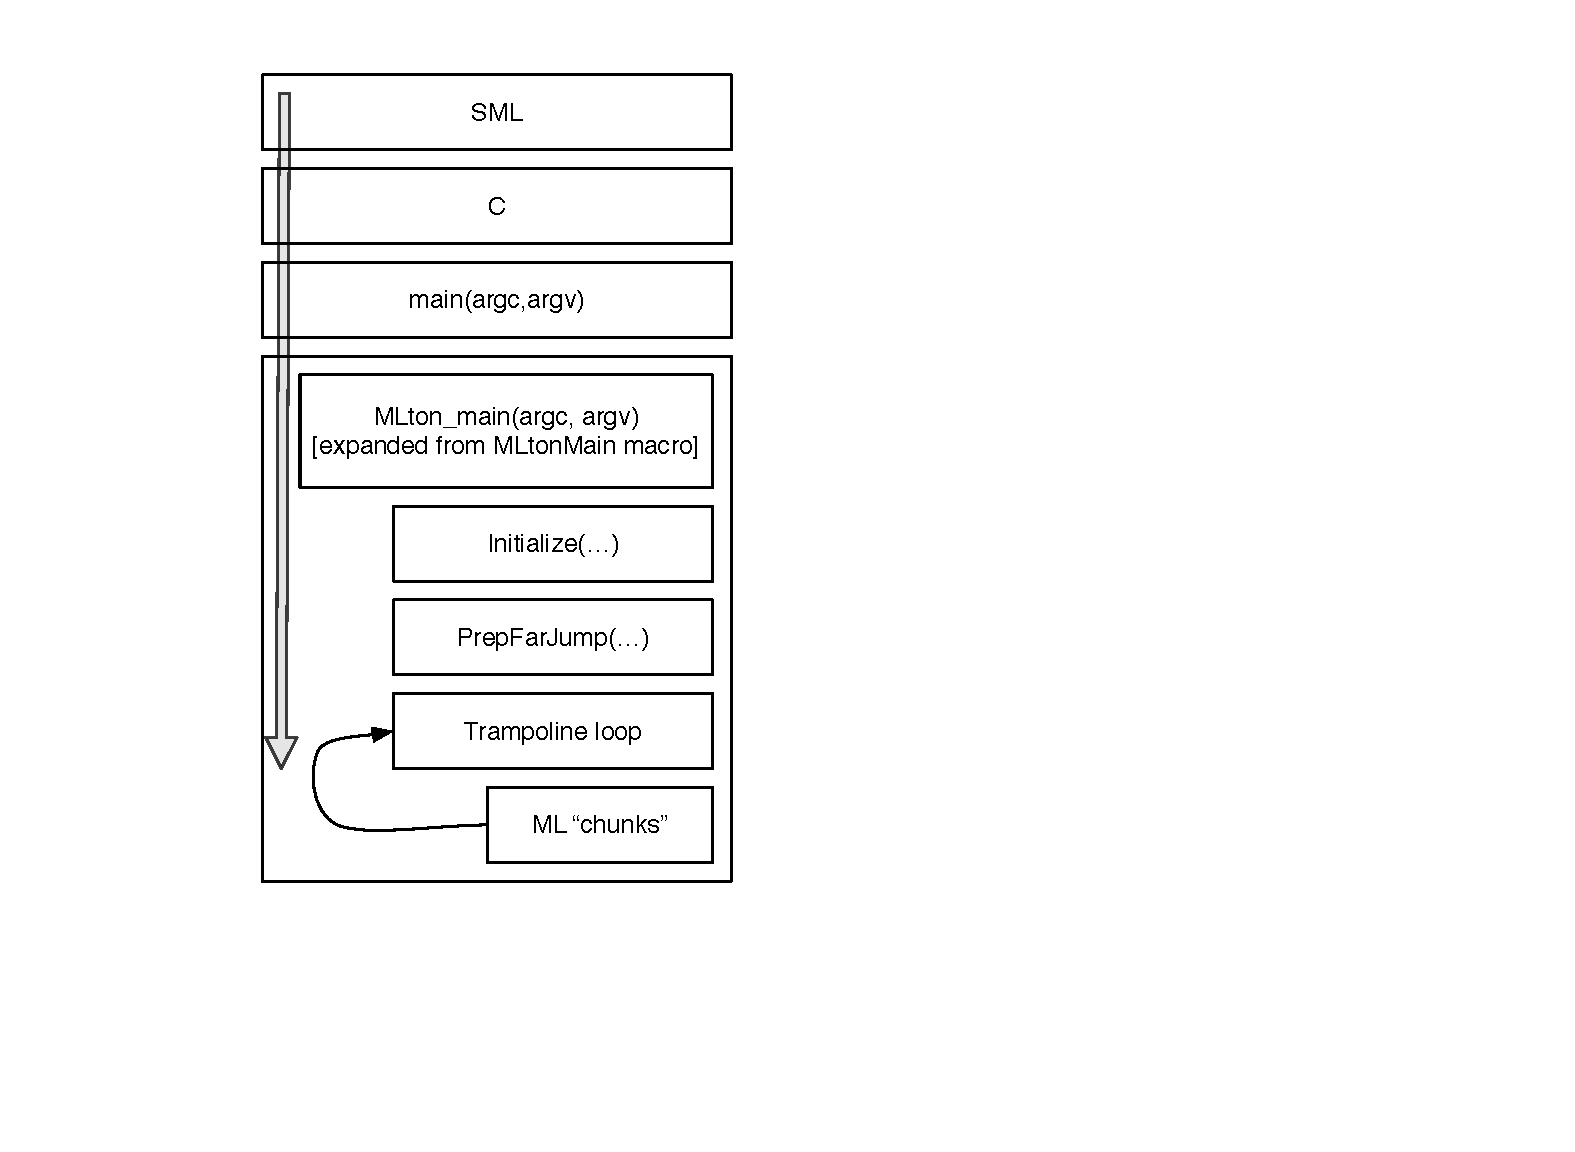
\epsfig{file=runtime-bootstrap-overview.pdf,width=2.0in}}
\figEnd{Runtime overview}{rtoverview}
       
When you compile your SML code, it is translated to machine code using one of several backends. For an in-depth description of how SML is compiled and optimized refer to~\cite{leibig:mlton-llvm-backend}. We will look at the C translation of a trivial SML program starting at the backend once all optimization phases have completed. The trivial SML program is a single statement: \texttt{val a = 2}

Refer to Figure~\ref{figure:rtoverview} for an overview of how the compiler emits C code given SML code, and how control flows through the bootstrap process of the emitted code.

 
The emitted C code bootstrap looks like this:

\lstset{language=C}\begin{lstlisting}
MLtonMain (8, 0x7CB29B69, 136, TRUE, PROFILE_NONE, FALSE, 0, 218)
int main (int argc, char* argv[]) {
    return (MLton_main (argc, argv));
}
\end{lstlisting}

\noindent and contains a \texttt{main} routine that calls \texttt{MLton\_main} which is created when the \texttt{MLtonMain} macro is expanded. 
\texttt{MLtonMain} is defined in \texttt{include/c-main.h} as a macro:

\lstset{language=C}\begin{lstlisting}
#define MLtonMain(al, mg, mfs, mmc, pk, ps, mc, ml)	
\end{lstlisting}

and ultimately calls the routine \texttt{MLton\_main (int argc, char* argv[])} which 

The parameters to the \texttt{MLtonMain} macro are:

\setlist[description]{leftmargin=!,labelindent=\parindent,labelwidth=1.5cm}

\begin{description}
\item[al] alignment width (\texttt{-align})
\item[mg] a magic random number used for saving/restoring the world. This number is generated at compile time by \texttt{mlton/codegen/c-codegen/c-codegen.fun} and allows the application to save and restore its state (\htmladdnormallink{MLtonWorld}{http://mlton.org/MLtonWorld})
\item[mfs] the maximum frame size
\item[mmc] whether or not the mutator marks cards. This is an optimization strategy used by the generational GC.
\item[pk] the kind of profiling to perform (compile time option)
\item[ps] whether stack profiling is enabled (\texttt{-profile-stack})
\item[mc] the number of the first chunk to jump to
\item[ml] the function number in the chunk to jump to
\end{description}

The first six of these parameters are passed to \texttt{Initialize} (defined in \texttt{include/common-main.h}) while the final two (mc and ml) are passed to \texttt{PrepFarJump} (defined in \texttt{include/c-common.h}). 
\texttt{Initialize} sets variables in the \texttt{gcState} structure and then calls \texttt{MLton\_init(argc, argv, \&gcState)}.



\texttt{MLton\_init} (\texttt{runtime/platform.c}) initializes the posix environment, the GC and processes the runtime command line arguments.  Once \texttt{Initialize} completes, \texttt{MLton\_main} continues and calls \texttt{PrepFarJump} to prepare to jump to the first chunk of the SML program. Alternatively, it will restore the saved world and restart from where the saved program left off. Finally, \texttt{MLton\_main} goes into an infinite loop, jumping from chunk to chunk as the SML program executes.
